\title{State Space Reduction For Parity Automata}
\author{Andreas Tollkötter}
\date{\today}

\pagestyle{empty}
\begin{titlepage}
\begin{center}
	\vspace*{\fill}
		\LARGE Rheinisch-Westfälische Technische Hochschule Aachen \\
	\vspace*{1cm}
		\LARGE Lehrstuhl für Informatik 7 \\
		\Large Logik und Theorie diskreter Systeme \\
	\vspace*{2cm}
		\LARGE Master Thesis \\
	\vspace*{5mm}
		\huge \textbf{State Space Reduction For Parity Automata} \\
	\vspace*{1cm}
		\Large by Andreas Tollkötter \\
	\vspace*{5mm}
		\Large 1st Supervisor: Priv.-Doz.\ Dr.\ Christof Löding \\
		\Large 2nd Supervisor: Prof.\ Dr.\ Joost-Pieter Katoen \\
	\vspace*{2cm}
		\large \today 
	\vspace*{\fill}
\end{center}
\end{titlepage}



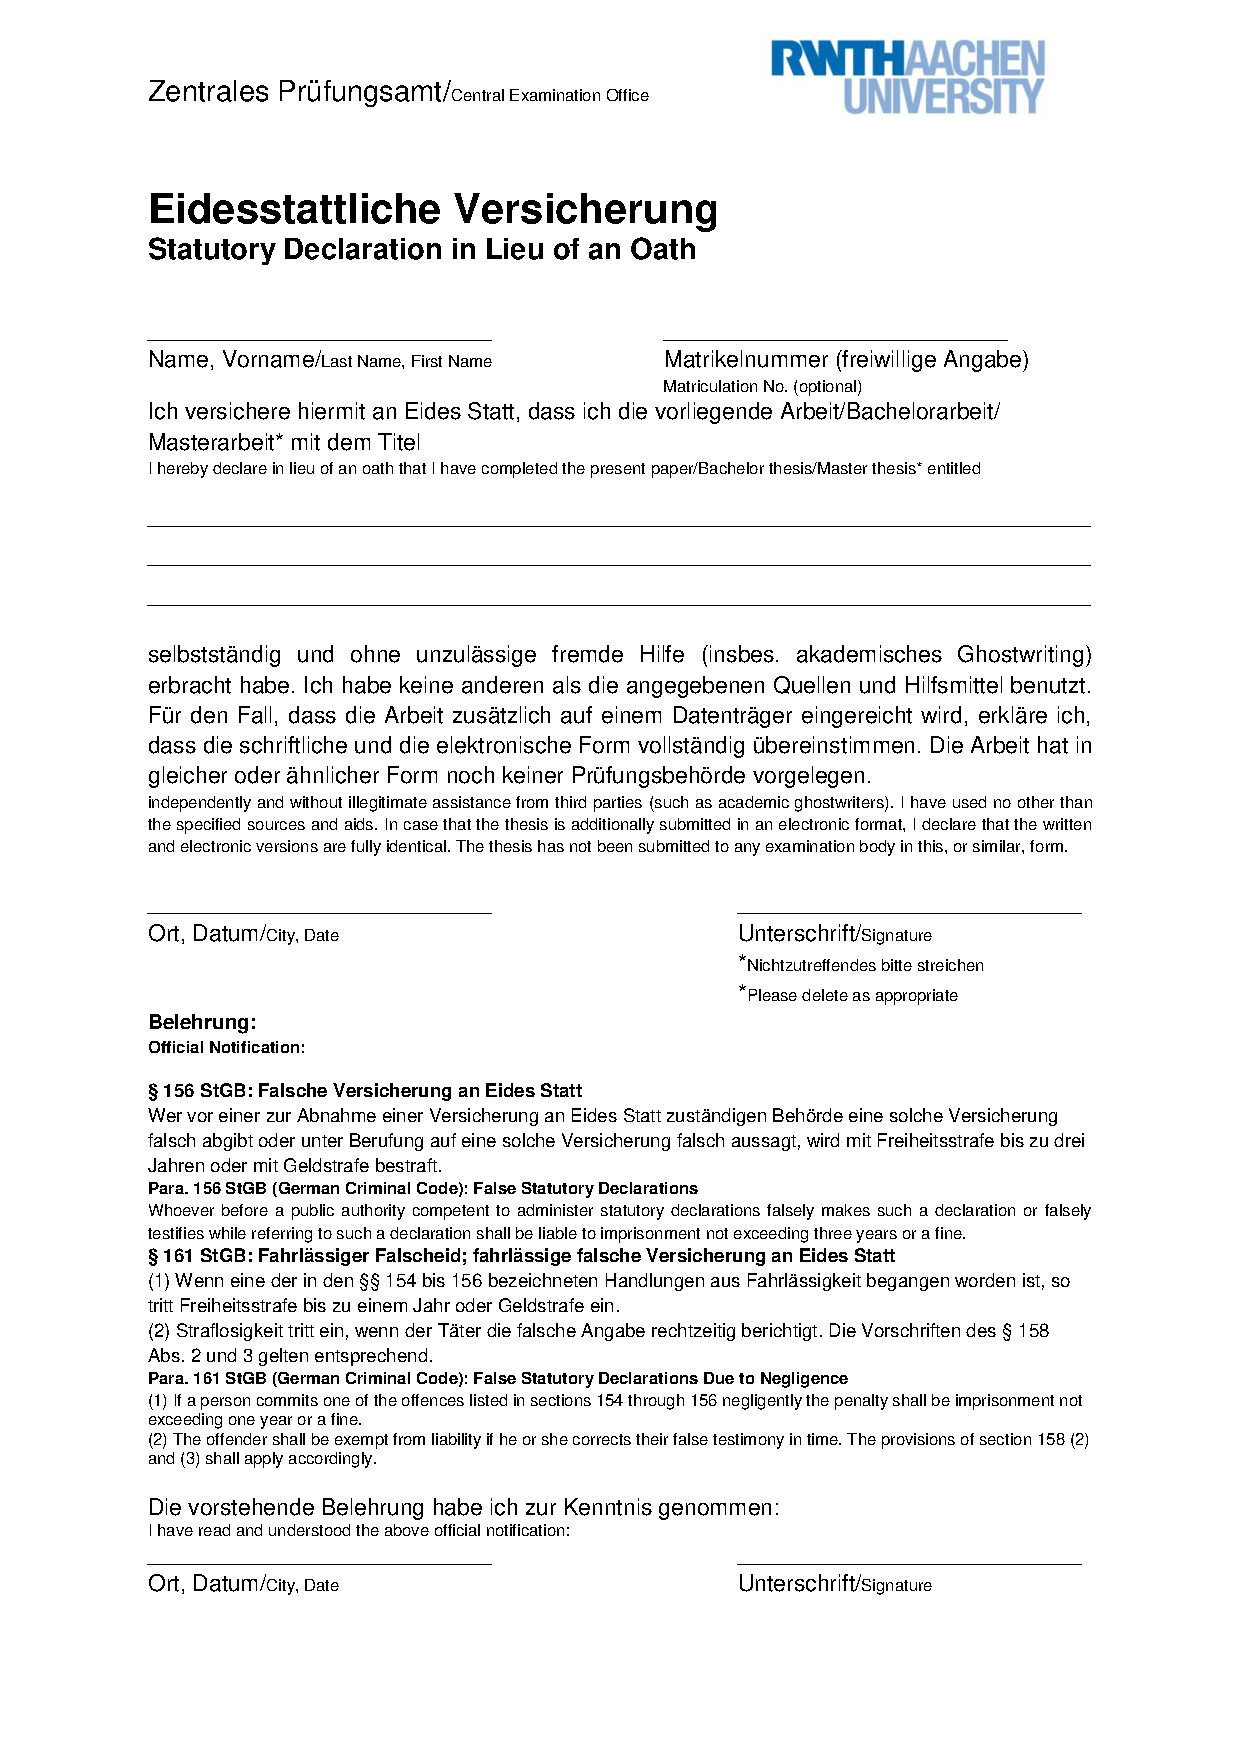
\includepdf{Formular_Eidesstattliche+Versicherung_neu}



\chapter*{Abstract}
Exact minimization of $\omega$-automata is a difficult problem and heuristic algorithms are a subject of current research. We establish a framework to generalize the known notion of quotient automata and uniformly describe such algorithms. We investigate several approaches to reduce the state space of deterministic parity automata. These are based on extracting information from structures within the automaton, such as strongly connected components, coloring of the states, and equivalence classes of given relations, to determine states that can safely be merged. The description of these procedures consists of a theoretical analysis as well as data collected from experiments.

%\clearpage
%\hbox{}
%\vspace{5cm}
%\section*{Acknowledgements}
%TODO
%I would like to thank my supervisor, Dr.\ Christof Löding, for his general help and knowledge regarding my thesis, my brother Alexander Tollkötter and my friend Niklas Rieken, for proof-reading, and Alexander Reeh, Tuan Nguyen, Michael Schletter, and Kathrin Tollkötter for personal support.



\fancypagestyle{plain}{%
  \fancyhf{}                          % clear all header and footer fields
  \renewcommand{\headrulewidth}{0pt}
  \renewcommand{\footrulewidth}{0pt}
}
\setcounter{tocdepth}{1}
\tableofcontents




\pagestyle{headings}

\newpage\null\thispagestyle{empty}\newpage
\section*{Introduction}

Finite automata are a long established computation model that dates back to sources such as \cite{McCulloch1990} and \cite{RabinScott1959}. A known problem for finite automata is state space reduction, referring to the search of a language-equivalent automaton which uses fewer states than the original object. For deterministic finite automata (DFA), not just reduction but minimization was solved in \cite{Hopcroft1971}. Regarding nondeterministic finite automata (NFA), \cite{JianRavikumar1991} proved the PSPACE-completeness of the minimization problem, which is why reduction algorithms such as \cite{ChamparnaudCoulon2004} and \cite{BonchiPous2013} are a popular alternative.

In his prominent work \cite{Buchi1966}, B\"uchi introduced the model of B\"uchi automata (BA) as an extension of finite automata to read words of one-sided infinite length. As these $\omega$-automata tend to have higher levels of complexity in comparison to standard finite automata, the potential gain of state space reduction is even greater. Similar to NFAs, exact minimization for deterministic B\"uchi automata was shown to be NP-complete in \cite{Schewe2010} and spawned heuristic approaches such as \cite{Schewe2010}, \cite{MayrClemente2012}, or \cite{EtessamiWilkeSchuller2001}. 

As \cite{Thomas1991} displays, deterministic B\"uchi automata are a strictly weaker model than nondeterministic Büchi automata. It is therefore interesting to consider different models of $\omega$-automata in which determinism is possible while maintaining enough power to describe all $\omega$-regular languages. Parity automata (PA) are one such model, a mixture of B\"uchi automata and Moore automata (\cite{Moore56}), that use a parity function rather than the usual acceptance set. \cite{Piterman2007} showed that deterministic parity automata are in fact sufficient to recognize all $\omega$-regular languages. As for DBAs, the exact minimization problem for DPAs is NP-complete (\cite{Schewe2010}).

Our goal in this publication is to develop new algorithms for state space reduction of DPAs, partially adapted from existing algorithms for B\"uchi or Moore automata. We perform theoretical analysis of the algorithms in the form of proofs of correctness and analysis of run time complexity, as well as practical implementation of the algorithms in code to provide empirical data for or against their actual efficiency.
